\chapter{引言}\label{sec:introduction}
\section{研究背景}

投资者评价一笔投资时，眼前的账户余额并不是唯一依据。设两位投资者的初始财富都为$1$，期末都为$1.2$：一人的账户曾升至$1.4$后回落，另一人曾跌至$0.8$后回升。前者可能觉得自己损失了已经到手的收益，后者则可能觉得已经摆脱亏损。两条路径的起点和终点相同，但经历改变了他们用来判断盈亏的参考点。若投资组合策略只观察期末财富，便无法区分这两种处境，也难以解释下一次调仓为何不同。

累积前景理论（cumulative prospect theory，CPT）以参考点为界评价收益和损失，并通过非线性的概率权重描述人们对不同风险事件的感受\citep{kahneman1979prospect,tversky1992advances}。在投资组合问题中，这意味着策略的好坏不仅取决于平均收益，还取决于各条财富路径的相对结果及其分布。强化学习使策略能够在连续决策中根据交互结果调整参数；CPT则为这种学习提供了不同于期望收益最大化的评价准则。已有工作研究了CPT下的预测、控制与有限时域策略梯度，为优化这类分布型目标提供了基础\citep{prashanth2016cumulative,lepel2026policygradients}。

然而，连续投资中的参考点不会始终停在买入价或预设常数上。证券交易实验发现，经历收益和损失后，人们会调整评价后续结果的基准，而且两个方向的调整幅度可能不同\citep{arkes2008reference}。适应性参考点与处置效应的关系、以及参考点对完整财富路径的依赖，也已在投资决策模型中得到研究\citep{he2019realization,qin2022realization}。当这些行为机制进入在线投资组合学习时，策略影响财富，财富改变参考点，参考点又改变下一期策略面对的CPT目标。即使外部市场条件暂时不变，投资者自己的交易经历也可能使目标发生移动；市场变化则会在此之外带来另一层扰动。

这一反馈使问题具有两个不同的难点。给定一期的市场和参考状态，CPT梯度中的概率权重仍依赖未知的结果分布，直接用有限轨迹的经验分布代替，通常会留下估计偏差。跨期来看，策略还须在目标随市场与账户状态变化时持续更新，不能只证明它在某一个固定目标附近停止。前一问题关乎有限轨迹能否提供可靠的一阶信息，后一问题关乎这些信息能否帮助策略跟上正在移动的目标。本文以动态参考点下的投资组合选择为场景，将二者放在同一在线优化问题中研究。

\section{文献综述}\label{sec:related}

\subsection{累积前景理论与策略优化}

前景理论及其累积形式把参考依赖的价值判断和非线性概率权重引入风险决策\citep{kahneman1979prospect,tversky1992advances}。一笔投资的结果先被判为相对于参考点的收益或损失，再经价值函数和概率权重进入评价。因而，两个平均收益相同的策略，只要极端亏损出现的概率不同，就可能得到不同的CPT价值。在多期投资中，评价对象是整条交易路径形成的终端结果分布；简单地把逐日收益换成另一种单期奖励，不能得到同一个目标。

围绕这一分布型目标，Prashanth等研究了CPT强化学习中的价值估计与控制，用经验结果分布计算CPT价值，再据此改进决策\citep{prashanth2016cumulative}。Lepel和Barakat则直接处理有限时域策略的参数优化：他们推导CPT策略梯度，将轨迹结果的顺序统计量用于蒙特卡洛估计，并分析所得策略达到近似驻点所需的样本量\citep{lepel2026policygradients}。前者说明了如何由样本评价一个具有概率加权的策略，后者进一步说明了如何利用轨迹样本调整策略参数。不过，一旦总体生存概率被有限样本的经验频率代替，非线性权重导数一般不会保持严格无偏；这一点在每期只能取得有限轨迹的在线学习中尤为重要。

投资组合领域还从另一条路线研究CPT目标。Luxenberg等利用目标的优化结构求解非凹的组合配置问题\citep{luxenberg2024portfolio}；Cui等和Wu等以交替方向方法处理概率加权目标及组合约束\citep{cui2025decision,wu2026behavioral}。这些方法着重于给定收益分布或给定决策问题时如何找到配置。本文沿用有限时域策略梯度的学习路线，关注的是每次调仓只能依据当期轨迹估计梯度、下一次调仓的参考点又会改变的情形。于是，有限样本梯度的统计性质与跨期目标的移动需要一并处理。

\subsection{动态参考点、路径依赖与投资者行为}

参考点如何随经历改变，首先是一个可以观察的行为问题。Arkes等在证券交易实验中发现，经历上涨后形成的收益基准与经历下跌后的调整并不对称；即使把股票放入组合情境，这种调整也仍值得考察\citep{arkes2008reference}。如果投资者曾见到账户升至较高水平，随后即便回落至买入价之上，也可能把这次回落视为损失。这说明固定买入成本不能概括投资者的全部盈亏判断。

实现效用研究把这种判断纳入动态交易模型。He和Yang研究单只股票的卖出与再次买入，允许参考点在盈利和亏损后以不同速度适应，说明参考点调整会改变盈利出售概率与亏损出售概率\citep{he2019realization}。Qin等进一步研究路径依赖的参考点：当前价格与当前持仓相同，先前经历过的高点或低点仍可能改变接下来的卖出选择\citep{qin2022realization}。从单只股票走向多期组合后，Gao等表明动态参考点和跨期相关的收益会共同影响配置决策\citep{gao2024multiperiod}。这些模型说明了历史经历为什么会进入当期选择，但其主要任务不是用轨迹样本估计CPT策略梯度，也不分析策略持续更新时目标如何随账户状态移动。

实际交易还提醒我们区分个股盈亏与整个组合的状态。组合整体的盈亏会影响投资者对个股的处置\citep{an2024portfolio}；有关中国投资者的研究则将社交媒体信息与处置行为联系起来\citep{chen2025xueqiu}。因此，同一只账面盈利股票是否被减持，不能只由一种参考点划分来解释。本文在比较静态、对称和非对称参考点时，使用同一批持股决策与相同的可观察控制变量，检验哪种盈亏表示更贴近实际减持。行为证据回答参考点是否有解释力；策略分析则回答参考点逐日变化后，投资组合如何学习。

\subsection{非平稳非凸在线优化与局部跟踪}

当市场条件每期改变时，策略面对的是一列目标函数。对非凸目标，即使知道每期的完整函数，也未必能以有限计算找到全局最优组合；要求在线策略始终追随这些最优组合，与梯度更新能够提供的保证并不相称。Aydore等为非凸在线预测提出动态局部遗憾，通过近期目标的一阶信息及其时间平滑，评价决策是否持续停留在局部不稳定的位置\citep{aydore2019dynamic}。这把关注点从“每期是否全局最优”转到“局部一阶偏差是否随时间积累”。

投资组合参数还受到可行域约束。位于边界的参数即使有非零梯度，也可能已经不能沿可行方向继续改善目标，因此直接累计梯度范数会误判其一阶状态。梯度映射与投影梯度研究为此采用投影后的一阶残差\citep{hallak2025sound,lan2026projected}。非平稳强化学习的变化预算进一步表明，目标变化越快，学习者越难仅凭有限样本保持跟踪精度\citep{feng2023nonstationary}。本文以当期真实CPT目标的投影残差描述可行的一阶偏差，再平滑最近各期的残差向量并累加其平方范数。外部市场改变收益规律，已执行策略改变财富与参考点；这两种来源一起进入目标变化预算，使在线界能够对应到投资过程本身。

\subsection{梯度去偏与因子化投资组合策略}

即使市场和期初参考点都已固定，CPT梯度仍包含未知的生存概率：需要知道一条轨迹的结果相对于其他可能结果处于什么位置，才能计算概率权重的边际作用。顺序统计量提供了可计算的样本近似\citep{lepel2026policygradients}，但将样本频率代入非线性函数，通常不能仅凭样本平均保证无偏。Rhee和Glynn的随机层级方法提供另一种思路：把不同精度估计之间的差分随机求和，在控制层级成本与差分波动时恢复目标量的期望\citep{rhee2015unbiased}。本文据此先用留一统计量避免轨迹参与自身的分位估计，再耦合全样本与两个半样本以消去主要波动。随机层修正消除剩余偏差，使每期得到的梯度估计能够与跨期在线更新的误差界衔接。

多资产投资还要求策略的每次输出都满足现金与股票权重非负、总和为一。André 和Coqueret以Dirichlet分布构造因子驱动的随机组合，资产特征通过浓度参数影响组合分配；这种参数化让同一组因子系数作用于所有股票，而每只股票因特征不同获得不同权重\citep{andre2021dirichlet}。它适合用策略梯度学习，但股票因子及其可用日期必须与交易顺序一致。中国A股的因子研究与动态金融数据集研究分别提供了市场特征和时间顺序处理的背景\citep{hanauer2024factor,liu2024dynamicdatasets}。本文保留这一可行的随机动作结构，在半合成市场中分别检验梯度估计与在线跟踪，再用真实A股价格路径考察投资后果。

\subsection{投资建议与异质投资者}

投资组合算法最终给出的并非抽象的目标值，而是一份现金与股票的具体配置建议。投资者可能愿意尝试某份建议，但执行后的感受仍取决于原有持仓、风险偏好和其间的价格路径。关于智能体风险偏好的研究指出，不同个体对相同风险结果的评价可能不同\citep{liu2025riskpreferences}；个性化投资顾问研究也将投资者差异纳入推荐过程\citep{takayanagi2025financialadvisors}。这些工作提示，推荐是否被接受与接受后的评价应分别观察。本文依据真实历史行为校准模拟投资者类型，使不同类型面对同一组组合建议，并以维持原持仓为对照计算采纳后的模型前景评价。这样可以观察建议在持续交互中的差异，同时保留真实投资者行为数据与模拟评价之间的区别。

\section{研究问题与贡献}

沿着上述研究脉络，本文的核心问题是：当投资者以随财富路径变化的参考点评价风险，而市场条件也在变化时，能否用有限轨迹可靠地估计每期CPT策略梯度，并使在线策略跟踪随之移动的一阶目标？这一问题包含相接的三个环节。首先，在给定期初状态和模拟模型后，需要知道有限样本梯度究竟指向哪个目标，以及估计误差如何随轨迹预算变化。其次，参考点和市场共同推动目标移动时，需要衡量持续更新能否减小当期的一阶残差，而不把固定目标下的收敛误认为移动目标下的跟踪。最后，若动态参考点确实承载投资经历的信息，它在组合决策和投资者实际卖出行为中应当留下可以观察的差别。

为回答这一问题，本文建立动态参考点下的CPT投资组合模型，并提出相应的在线策略梯度方法DRCPT-PG。策略用资产因子决定Dirichlet分布的浓度，从中随机生成现金与股票的组合。每期开始时，多条模拟路径与真实账户共享同一个已知状态；此后参考点沿各自的每日财富变化更新，期末财富相对期末参考点的结果进入CPT评价。这样，策略参数影响的不仅是当期投资权重，也通过财富路径影响未来的评价基准。

统计分析先固定一期目标。正则化CPT的得分梯度恒等式说明如何把轨迹在结果分布中的位置与策略得分结合；中心化留一估计和随机层级修正则使有限轨迹下的梯度输出严格无偏，同时具有有限方差和有限期望轨迹成本。本文进一步给出其渐近正态性，以及固定维度下最优的轨迹预算速率。跨期分析转向不断移动的目标：归一化投影更新的残差界分别计入目标变化、轨迹估计误差和模拟模型误差；近期残差经时间平滑后得到动态局部遗憾界。在附加的局部误差界条件下，残差还控制参数到当期驻点集合的距离。

实验先在受控市场中检验这些环节：相同期末财富能否因路径不同而改变配置选择；有限轨迹给出的梯度有多准；目标连续移动时，更新策略是否比冻结参数更接近当期一阶条件。参考点适应速度、时期长度和更新尺度随后分别变化，以观察跟踪结果如何改变。再把方法放入时间顺序的沪深300回放，看收益、风险和交易成本；用真实持股决策比较三种参考点对减持行为的样本外解释力；最后在历史行为校准的模拟投资者中，分别观察推荐是否被采纳及采纳后的模型评价。图~\ref{fig:research-framework}概括了这些问题之间的关系。

\begin{figure}[htbp]
    \centering
    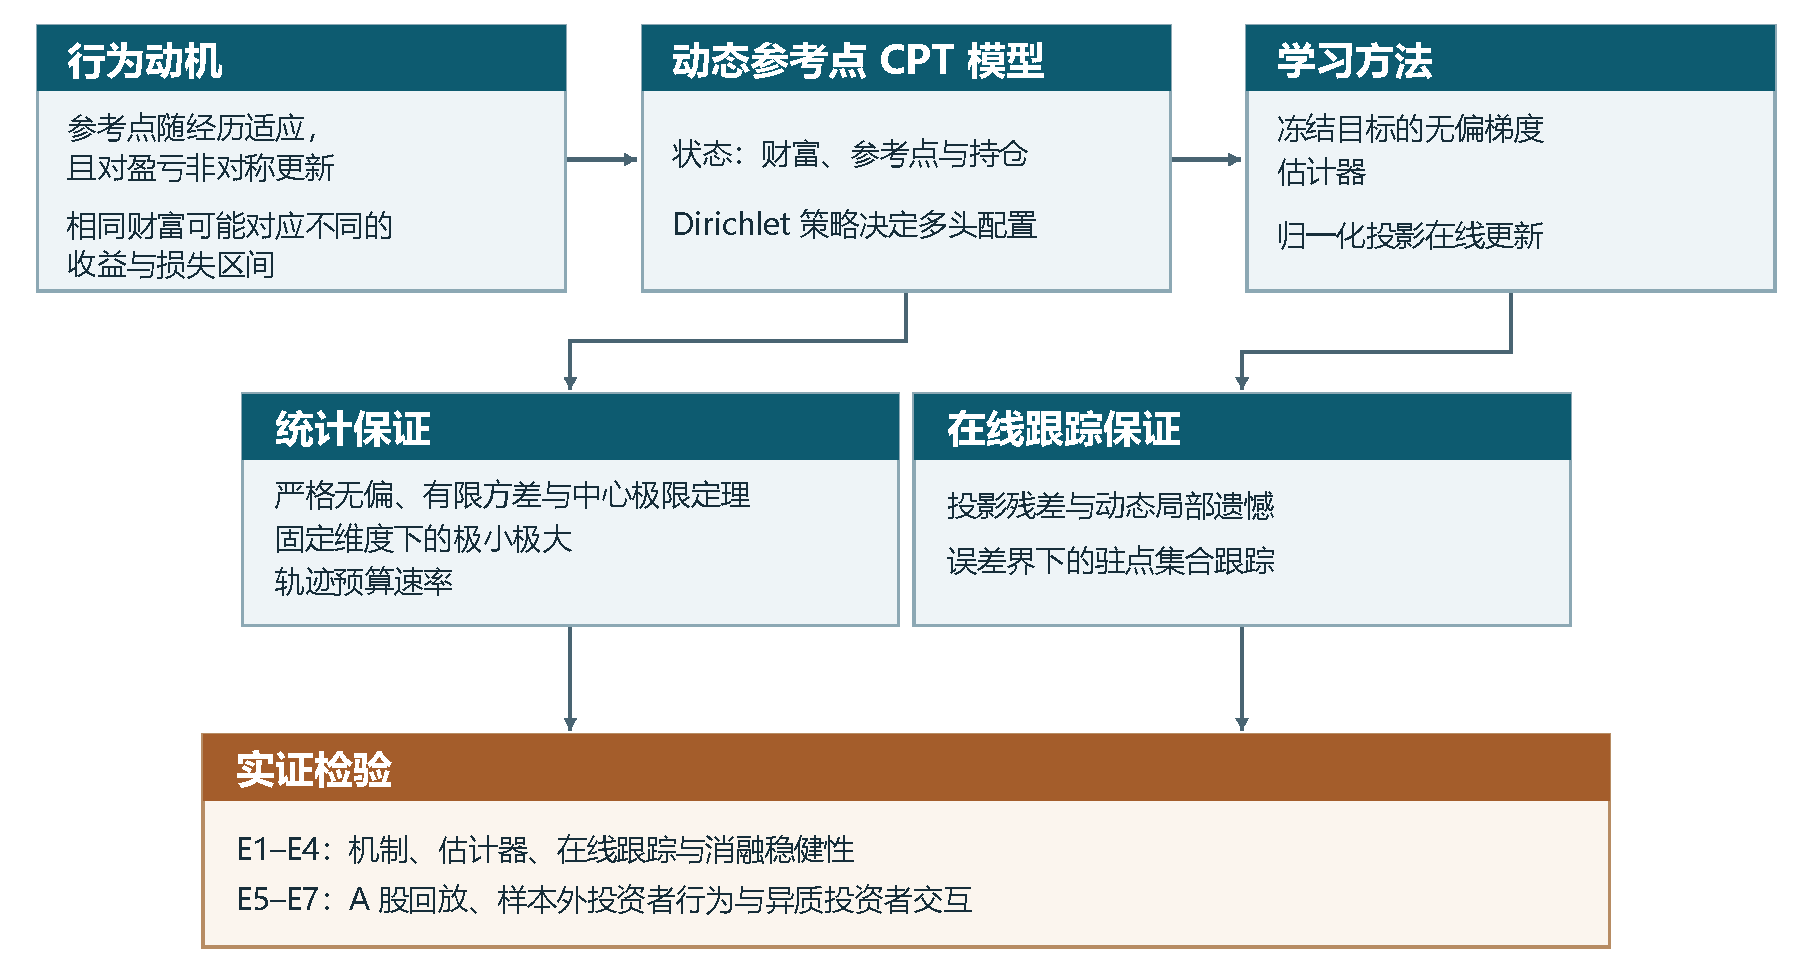
\includegraphics[width=0.96\textwidth]{figures/research_framework_zh.pdf}
    \caption{本文研究框架}
    \label{fig:research-framework}
\end{figure}

\section{论文结构}

第二章给出问题设定与假设，第三章介绍梯度估计和在线更新，第四章证明估计性质及跟踪界。第五章通过七项实验连接可控机制、A股回放与投资者行为，第六章讨论主要发现；相关证明收于附录。
